\documentclass{article}
\usepackage{graphicx} % Required for inserting images
\usepackage{geometry}
\geometry{a4paper, margin=0.5in}
\usepackage{longtable}
\usepackage{amsmath}
\usepackage{arydshln}
\usepackage{amssymb}
\allowdisplaybreaks
\usepackage{mathtools}
\usepackage{gensymb}

\title{NuScale Homework}
\author{Olin Calvin}
\date{July 2023}

\begin{document}

\maketitle

\section{Question 1}

Answer: $T_{s,2} = 253 \degree$F

\begin{figure}[htbp]
    \centering
    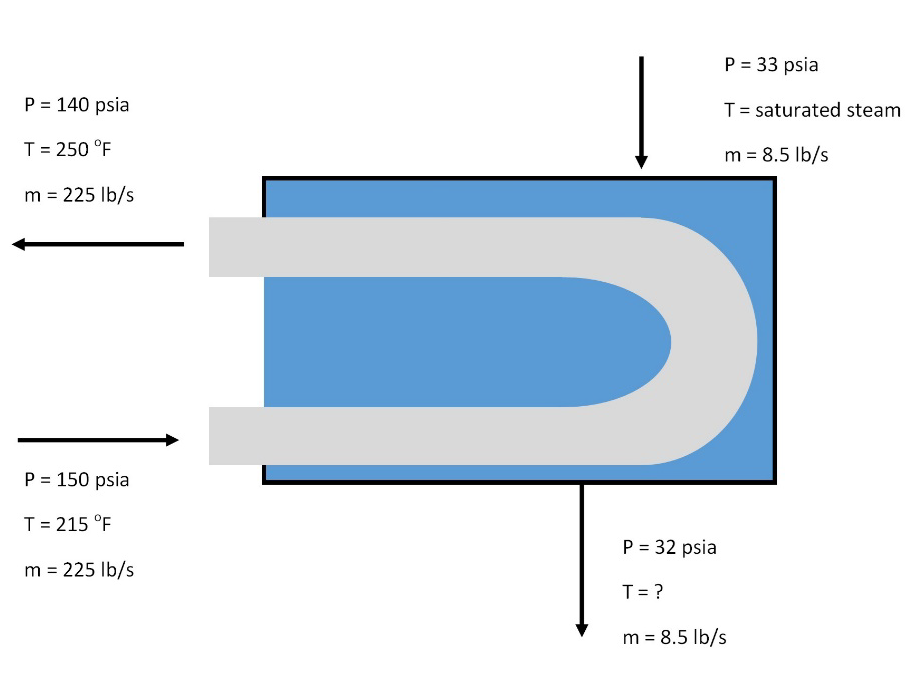
\includegraphics[width=0.75\textwidth]{question_1_picture.png}
    \caption{Determine the outlet temperature of the shell side of a shell and tube heat exchanger given here.}
    \label{fig:question_1_fig}
\end{figure}

Use subscript t for the tube side and s for the shell side.

Knowns:

\begin{align*}
    P_{t,1} &= 150 \text{ psia} \\
    m_{t,1} = m_{t,2} &= 225 \frac{\text{lb}}{\text{s}} \\
    P_{t,2} &= 140 \text{ psia} \\
    T_{t,1} &= 215 \degree \text{F} \\
    T_{t,2} &= 250 \degree \text{F} \\
    P_{s,1} &= 33 \text{psia} \\
    P_{s,2} &= 32 \text{psia} \\
    T_{s,1} &= \text{saturation temperature} \\
    x_{s,1} &= 1.0 \\
    m_{s,1} = m_{s,2} &= 8.5 \frac{\text{lb}}{\text{s}}
\end{align*}

Can determine the enthalpy of at $t,1$, $t,2$, and $s,1$ via steam tables. Will use Table E.1 from \textit{Nuclear Systems Volume 1 Thermal Hydraulic Fundamentals Second Edition} by N. Todreas and M. Kazimi.

For convenience, will convert units to metric, which Table E.1 is in.

\begin{align*}
    P_{t,1} &= 1.034 \text{ MPa} \\
    m_{t,1} = m_{t,2} &= 102 \frac{\text{kg}}{\text{s}} \\
    P_{t,2} &= 0.965 \text{ MPa} \\
    T_{t,1} &= 101.67 \degree \text{C} \\
    T_{t,2} &= 121.11 \degree \text{C} \\
    P_{s,1} &= 0.2275 \text{ MPa} \\
    P_{s,2} &= 0.2206 \text{ MPa} \\
    T_{s,1} &= \text{saturation temperature} \\
    x_{s,1} &= 1.0 \\
    m_{s,1} = m_{s,2} &= 3.856 \frac{\text{kg}}{\text{s}}
\end{align*}

Determine the enthalpy of the known states. Use a spreadsheet to calculate the interpolated points of Table E.1. Additionally, I will assume that all liquids are saturated because the impact of varying pressure on liquids is relatively low and the pressure changes here are not remarkably large.

The saturation temperature of 140 psia is over 300 $\degree$F so the tube side is always a liquid.

In metric, the tube side has the following enthalpies (calculated via linear interpolation of Table E.1)

\begin{align*}
    h_{t,1} &= 426.2 \frac{\text{kJ}}{\text{kg}} \\
    h_{t,2} &= 508.5 \frac{\text{kJ}}{\text{kg}} \\
    \Delta h_t = h_{t,2} - h_{t,1} &= 508.5 \frac{\text{kJ}}{\text{kg}} - 426.2 \frac{\text{kJ}}{\text{kg}} = +82.3 \frac{\text{kJ}}{\text{kg}}
\end{align*}

Can now calculate the increase in enthalpy of the tube side

\begin{equation}
    m_t \Delta h_t = 102 \frac{\text{kg}}{\text{s}} \times 82.3 \frac{\text{kJ}}{\text{kg}} = 8395 \frac{\text{kJ}}{\text{s}}
\end{equation}

Now the enthalpy change over time can be used to inform the decrease in enthalpy on the shell side.

\begin{align*}
    T_{s,1} &= 124 \degree C \\
    h_{s,1} &= 2711.6 \frac{\text{kJ}}{\text{kg}}
\end{align*}

Now we can use the mass flow rate through the shell side to determine the enthalpy of $s,2$

\begin{align}
    m_s \Delta h_s = -m_t \Delta h_t &= -8395 \frac{\text{kJ}}{\text{s}} \\
    \Delta h_s &= \frac{-8395 \frac{\text{kJ}}{\text{s}}}{3.856 \frac{\text{kg}}{\text{s}}} \\
    \Delta h_s &= 2177 \frac{\text{kJ}}{\text{kg}}
\end{align}

Since the pressure of $s,2$ is known, the saturation temperature can be determined as well as the enthalpy of saturated liquid water at that pressure

\begin{align*}
    T_{\text{sat},s,2} &= 123 \degree \text{C} \\
    h_{\text{sat},l,s,2} &= 517 \frac{\text{kJ}}{\text{kg}}
\end{align*}

Calculate the enthalpy difference between $h_{s,1}$ and $h_{\text{sat},l,s,2}$. This is a good sanity check, because if the enthalpy difference between these two is smaller than the enthalpy change calculated that likely means I made a mistake somewhere.

\begin{equation}
    h_{s,1} - h_{\text{sat},l,s,2} = 2711.6 \frac{\text{kJ}}{\text{kg}} - 517 \frac{\text{kJ}}{\text{kg}} = 2194.6 \frac{\text{kJ}}{\text{kg}}
\end{equation}

Since the enthalpy change of $2177 \frac{\text{kJ}}{\text{kg}}$ is smaller than the enthalpy change between saturated vapor at $P_{s,1}$ and saturated liquid at $P_{s,2}$, it can be determined that the $s,2$ exit condition is mixture of liquid and vapor (but mostly liquid) and the temperature is the saturation temperature of $P_{s,2}$ which is $123 \degree$C or $253 \degree$F. This also makes sense physically as $T_{s,2}$ cannot be less than the temperature of $t,1$ and the pinch point of the heat exchanger must be positive.

Just for completeness, I'll calculate the exit quality.

\begin{align*}
    h_{\text{sat},l,s,2} &= 517 \frac{\text{kJ}}{\text{kg}} \\
    h_{\text{sat},g,s,2} &= 2710 \frac{\text{kJ}}{\text{kg}}
\end{align*}

\begin{equation}
    h_{s,2} = h_{s,1} - \Delta h_s = 2711.6 \frac{\text{kJ}}{\text{kg}} - 2177 \frac{\text{kJ}}{\text{kg}} = 534.6 \frac{\text{kJ}}{\text{kg}}
\end{equation}

\begin{equation}
    x_{s,2} = \frac{h_{s,2} - h_{\text{sat},l,s,2}}{h_{\text{sat},g,s,2} - h_{\text{sat},l,s,2}} = \frac{534.6 - 517}{2710 - 517} = 0.008
\end{equation}

With an exit quality of 0.008, the outlet of the shell side of the heat exchanger is close to, but not quite, saturated liquid.

\newpage

\section{Question 2}

Answer: TDH = 136.4 feet

\begin{figure}[htbp]
    \centering
    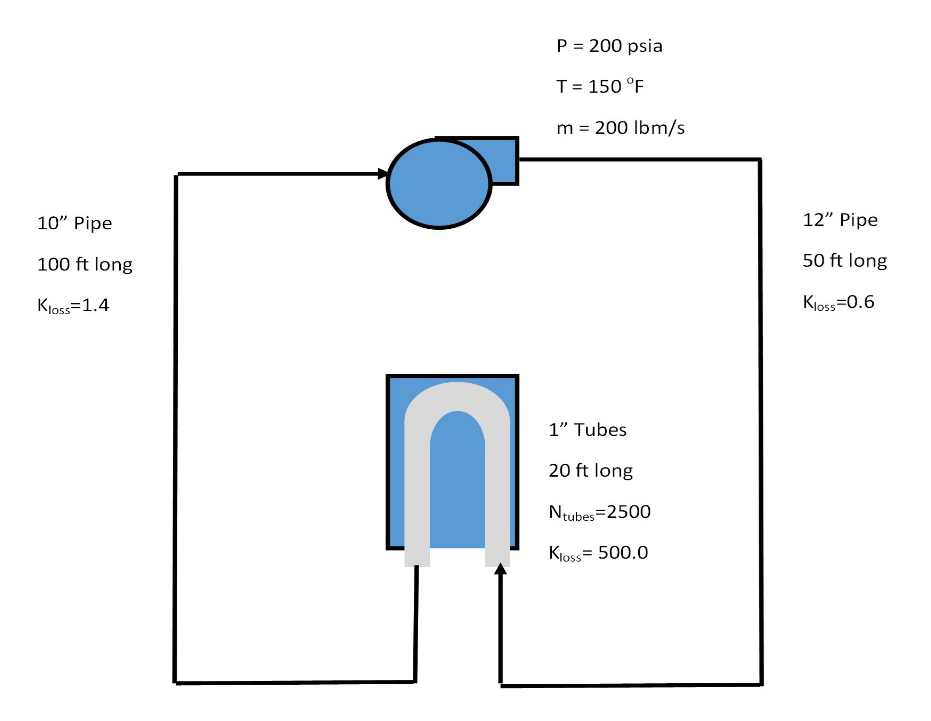
\includegraphics[width=0.75\textwidth]{question_2_picture.png}
    \caption{Determine the Total Dynamic Head required for the pump in the following flow loop. Assume that there is no temperature change over the heat exchanger and a friction factor, f=0.01.}
    \label{fig:question_2_fig}
\end{figure}

I'm going to assume the form loss hit is immediate at the beginning of each change in flow shape. I am also assuming that there's no elevation change here. Also assuming the flow is incompressible.

Going to be referring to Section 9.3.6 Pressure Drop in Channels from \textit{Nuclear Systems Volume 1 Thermal Hydraulic Fundamentals Second Edition} by N. Todreas and M. Kazimi.

Form loss can be calculated by Eq. 9.39d from T\&K. It is also assumed that for form loss, $v_{\text{ref}}$ is the larger of the two velocities on either side of the form loss.

\begin{equation}
    \Delta p_{\text{form}} = K \frac{\rho v_{\text{ref}}^2}{2}
\end{equation}

And friction loss can be calculated by Eq. 9.39e from T\&K with the assumption that $f = \overline{f}$.

\begin{equation}
    \Delta p_{\text{friction}} = f \frac{L}{D_{\text{e}}} \frac{\rho v_{\text{ref}}^2}{2}
\end{equation}

And acceleration loss can be calculated by Eq. 9.39b.

\begin{equation}
    \Delta p_{\text{acceleration}} = \frac{m^2}{2 \rho} (\frac{1}{A_N^2} - \frac{1}{A_1^2})
\end{equation}

I am once again converting metric because Table E.1 in T\&K is in metric

\begin{align*}
    T_p &= 150 \degree \text{F} = 65.56 \degree \text{C} \\
    P_p &= 200 \text{ psia} = 1.379 \text{ MPa} \\
    m_p &= 200 \frac{\text{lbm}}{\text{s}} = 90.7 \frac{\text{kg}}{\text{s}} \\
    D_1 &= 12 \text{ in} = 0.3048 \text{ m} \\
    L_1 &= 50 \text{ ft} = 15.24 \text{ m} \\
    D_2 &= 1 \text{ in} = 0.0254 \text{ m} \\
    L_2 &= 20 \text{ ft} = 6.096 \text{ m} \\
    D_3 &= 10 \text{ in} = 0.254 \text{ m} \\
    L_3 &= 100 \text{ ft} = 30.48 \text{ m}
\end{align*}

Calculate the density of water, based on Table E.1 $v = 1.020 \times 10^{-3} \frac{\text{m}^3}{\text{kg}}$. Invert to get the density of the water which is $\rho = \frac{1}{v} = 980.4 \frac{\text{kg}}{\text{m}^3}$

Now calculate flow areas and flow velocities for each region

\begin{align}
    A_1 &= \frac{\pi D_1^2}{4} = 0.07297 \text{ m}^2 \\
    v_1 &= \frac{m}{\rho A_1} = \frac{90.7 \frac{\text{kg}}{\text{s}}}{980.4 \frac{\text{kg}}{\text{m}^3} \times 0.07297 \text{ m}^2} = 1.2678 \frac{\text{m}}{\text{s}} \\
    A_2 &= N_{\text{tubes}} \frac{\pi D_2^2}{4} = 1.2668 \text{ m}^2 \\
    v_2 &= \frac{m}{\rho A_2} = \frac{90.7 \frac{\text{kg}}{\text{s}}}{980.4 \frac{\text{kg}}{\text{m}^3} \times 1.2668 \text{ m}^2} = 0.07303 \frac{\text{m}}{\text{s}} \\
    A_3 &= \frac{\pi D_3^2}{4} = 0.05067 \text{ m}^2 \\
    v_3 &= \frac{m}{\rho A_3} = \frac{90.7 \frac{\text{kg}}{\text{s}}}{980.4 \frac{\text{kg}}{\text{m}^3} \times 0.05067 \text{ m}^2} = 1.8258 \frac{\text{m}}{\text{s}}
\end{align}

I assume there has to be a point somewhere where the 10 inch pipe and the 12 inch pipe changeover. This results in form loss, and the larger of the two velocities will be used, thus $v_3$ is used for calculating form loss in the first region.

\begin{equation}
    \Delta p_{\text{form},1} = K_1 \frac{\rho v_{3}^2}{2} = 0.6 \frac{980.4 \frac{\text{kg}}{\text{m}^3} \times (1.8258 \frac{\text{m}}{\text{s}})^2}{2} = 980.5 \frac{\text{kg}}{\text{m} \cdot \text{s}^2} = 980.5 \text{ Pa}
\end{equation}

Now calculate the friction loss in region 1

\begin{equation}
    \Delta p_{\text{friction},1} = f \frac{L_1}{D_1} \frac{\rho v_1^2}{2} = 0.01 \frac{15.24 \text{ m}}{0.3048 \text{ m}} \frac{980.4 \frac{\text{kg}}{\text{m}^3} \times (1.2668 \frac{\text{m}}{\text{s}} )^2}{2} = 393.3 \text{ Pa}
\end{equation}

There are also acceleration changes as a result of changing flow area from $A_3$ to $A_1$

\begin{equation}
    \Delta p_{\text{acceleration},1} = \frac{m^2}{2 \rho} (\frac{1}{A_1^2} - \frac{1}{A_3^2}) = \frac{(90.7 \frac{\text{kg}}{\text{s}})^2}{2 \times 980.4 \frac{\text{kg}}{\text{m}^3}}(\frac{1}{(0.07297 \text{ m}^2)^2} - \frac{1}{(0.05067 \text{ m}^2)^2}) = -846.2 \text{ Pa}
\end{equation}

Negative indicates a pressure increase from the deceleration of the flow as expected.

Now calculate the form loss in region 2 (this will be big), use $v_1$ as the reference velocity

\begin{equation}
    \Delta p_{\text{form},2} = K_2 \frac{\rho v_{1}^2}{2} = 500 \frac{980.4 \frac{\text{kg}}{\text{m}^3} \times (1.2678 \frac{\text{m}}{\text{s}})^2}{2} = 393953.4 \text{ Pa}
\end{equation}

Friction loss next, since the pipes are parallel, we only need to calculate the friction loss in one tube which can be applied uniformly.

\begin{equation}
    \Delta p_{\text{friction},2} = f \frac{L_2}{D_2} \frac{\rho v_2^2}{2} = 0.01 \frac{6.096 \text{ m}}{0.0254 \text{ m}} \frac{980.4 \frac{\text{kg}}{\text{m}^3} \times (0.07303 \frac{\text{m}}{\text{s}} )^2}{2} = 6.3 \text{ Pa}
\end{equation}

And now the pressure change from acceleration which should be a large increase since the flow decelerates a lot

\begin{equation}
    \Delta p_{\text{acceleration},2} = \frac{m^2}{2 \rho} (\frac{1}{A_2^2} - \frac{1}{A_1^2}) = \frac{(90.7 \frac{\text{kg}}{\text{s}})^2}{2 \times 980.4 \frac{\text{kg}}{\text{m}^3}}(\frac{1}{(1.2668 \text{ m}^2)^2} - \frac{1}{(0.07297 \text{ m}^2)^2}) = -785.3 \text{ Pa}
\end{equation}

Not as large as the acceleration change in 1, which after writing it out makes more sense because the change is dictated by the magnitude of the inverse of the square of the area. The smallest the first inverse area term can be is close to zero meaning the potential acceleration increase is capped by the size of the second area.

Alright last one, for form loss use the larger term which is $v_3$

\begin{equation}
    \Delta p_{\text{form},3} = K_3 \frac{\rho v_{3}^2}{2} = 1.4 \frac{980.4 \frac{\text{kg}}{\text{m}^3} \times (1.8258 \frac{\text{m}}{\text{s}})^2}{2} = 2287.7 \text{ Pa}
\end{equation}

Friction loss next

\begin{equation}
    \Delta p_{\text{friction},3} = f \frac{L_3}{D_3} \frac{\rho v_3^2}{2} = 0.01 \frac{30.48 \text{ m}}{0.254 \text{ m}} \frac{980.4 \frac{\text{kg}}{\text{m}^3} \times (1.8258 \frac{\text{m}}{\text{s}} )^2}{2} = 1960.9 \text{ Pa}
\end{equation}

And now the pressure change from acceleration

\begin{equation}
    \Delta p_{\text{acceleration},3} = \frac{m^2}{2 \rho} (\frac{1}{A_3^2} - \frac{1}{A_2^2}) = \frac{(90.7 \frac{\text{kg}}{\text{s}})^2}{2 \times 980.4 \frac{\text{kg}}{\text{m}^3}}(\frac{1}{(0.05067 \text{ m}^2)^2} - \frac{1}{(1.2668 \text{ m}^2)^2}) = 1631.5 \text{ Pa}
\end{equation}

And the acceleration terms all cancel one another out, which I suspected but wanted to make sure.

Since the acceleration terms can be ignored it's a summation of the friction and form terms.

\begin{equation}
    980.5 + 393.3 + 393953.4 + 6.3 + 2287.7 + 1960.9 = 399582.1 \text{ Pa}
\end{equation}

Quick sanity check, the pressure drop is about 58 psia, meaning the pressure hasn't gone negative or any phase change has occurred (assuming the fluid is water).

Total Dynamic Head is given in units of length which represents the equivalent height the fluid needs to be pumped to overcome pressure losses

Assume this is occurring on Earth with standard gravity

\begin{align}
    \Delta p = 399582.1 \text{ Pa} &= \rho g (z_2 - z_1) = 980.4 \frac{\text{kg}}{\text{m}^3} \times 9.807 \frac{\text{m}}{\text{s}^2} (z - 0) \\
    \frac{399582.1 \frac{\text{kg}}{\text{m} \cdot \text{s}^2}}{980.4 \frac{\text{kg}}{\text{m}^3} \times 9.807 \frac{\text{m}}{\text{s}^2}} &= z \\
    z &= 41.56 \text{ m}
\end{align}

Convert to feet and the total dynamic head needed is 136.4 feet and is mostly driven by the massive form loss.

\newpage

\section{Question 3}

\begin{table}[htbp]
    \centering
    \begin{tabular}{|c|c|c|}
    \hline
    Property & Fuel & Cladding \\ \hline
    $k \frac{\text{W}}{\text{m} \cdot \text{K}}$ & 3.6 & 13.0 \\ \hline
    $\rho \frac{\text{kg}}{\text{m}^3}$ & 9670.0 & 6500.0 \\ \hline
    $c_p \frac{\text{J}}{\text{kg} \cdot \text{K}}$ & 247.0 & 330.0 \\ \hline
    $q''' \frac{\text{kW}}{\text{m}^3}$ & 1000.0 & 0.0 \\ \hline
    $L$ cm & 1.0 & 0.1 \\ \hline
    \end{tabular}
    \caption{Properties}
    \label{tab:q3_properties}
\end{table}

Left hand side is perfectly insulated. Right hand side is convective with convection coefficient $h = 120 \frac{\text{kW}}{\text{m}^2 \cdot \text{K}}$.

$T_{\infty} = 350 \degree$C 

\subsection{Analytical Solution at Steady-State}

The volumetric heat generation is 1000 $\frac{\text{kW}}{\text{m}^3}$ in the fuel, which is 1 cm thick. In order to be in steady-state, as much heat must be flowing out of the fuel, through the cladding, and into the coolant as is being generated. Used \textit{Fundamentals of Heat and Mass Transfer Seventh Edition} by T. Bergman, A. Lavine, F. Incropera, and D. Dewitt as a reference.

If it is assumed that the fuel-insulation interface corresponds to x=0 then the temperature distribution of the fuel rod can be calculated via

\begin{align}
    T_{\text{plate}} &= \frac{(q''' L_f)(L_c + L_f - x)}{k_c} + \frac{q''' L_f}{h} + T_{\infty}, 0.01 \text{ m} \leq x \leq 0.011 \text{ m} \\
    T_{\text{plate}} &= \frac{q''' L_f^2}{2 k_f}(1 - \frac{x^2}{L_f^2}) + \frac{(q''' L_f)(L_c)}{k_c} + \frac{q''' L_f}{h} + T_{\infty}, x \leq 0.01 \text{ m}
\end{align}


$T_co$ occurs when $x = 0.011$ m.

\begin{align}
    T_{co} &= \frac{(10^{6} \frac{\text{W}}{\text{m}^3} 0.01 \text{ m})(0.001 \text{ m} + 0.01 \text{ m} - 0.011 \text{ m})}{13 \frac{\text{W}}{\text{m} \cdot \text{K}}} + \frac{10^{6} \frac{\text{W}}{\text{m}^3} 0.01 \text{ m}}{1.2 \times 10^{5} \frac{\text{W}}{\text{m}^2 \cdot K}} + 350 \degree \text{C} \\
    T_{co} &= 350.083 \degree \text{C}
\end{align}

$T_{fci}$ occurs when $x = 0.01$ m.

\begin{align}
    T_{fci} &= \frac{(10^{6} \frac{\text{W}}{\text{m}^3} 0.01 \text{ m})(0.001 \text{ m} + 0.01 \text{ m} - 0.01 \text{ m})}{13 \frac{\text{W}}{\text{m} \cdot \text{K}}} + \frac{10^{6} \frac{\text{W}}{\text{m}^3} 0.01 \text{ m}}{1.2 \times 10^{5} \frac{\text{W}}{\text{m}^2 \cdot K}} + 350 \degree \text{C} \\
    T_{fci} &= \frac{(10^{6} \frac{\text{W}}{\text{m}^3} 0.01 \text{ m})(0.001 \text{ m} + 0.01 \text{ m} - 0.01 \text{ m})}{13 \frac{\text{W}}{\text{m} \cdot \text{K}}} + 350.083 \degree \text{C} \\
    T_{fci} &= 350.852 \degree \text{C}
\end{align}

$T_{fc}$ (fuel-center) occurs when $x=0.005$ m.

\begin{align}
    T_{fc} &= \frac{10^{6} \frac{\text{W}}{\text{m}^3} \times (0.01 \text{ m})^2}{2 \times 3.6 \frac{\text{W}}{\text{m} \cdot \text{K}}} (1 - \frac{(0.005 \text{ m})^2}{(0.01 \text{ m})^2}) + \frac{(10^{6} \frac{\text{W}}{\text{m}^3} 0.01 \text{ m})(0.001 \text{ m})}{13 \frac{\text{W}}{\text{m} \cdot \text{K}}} + \frac{10^{6} \frac{\text{W}}{\text{m}^3} 0.01 \text{ m}}{1.2 \times 10^{5} \frac{\text{W}}{\text{m}^2 \cdot K}} + 350 \degree \text{C} \\
    T_{fc} &= \frac{10^{6} \frac{\text{W}}{\text{m}^3} \times (0.01 \text{ m})^2}{2 \times 3.6 \frac{\text{W}}{\text{m} \cdot \text{K}}} (1 - \frac{(0.005 \text{ m})^2}{(0.01 \text{ m})^2}) + 350.852 \degree \text{C}\\
    T_{fc} &= 361.269 \degree \text{C}
\end{align}

Check the insulated wall temperature as well, which is calculated to be roughly $364.74 \degree$C which is to be expected as the fuel region should have a parabolic shape.

\end{document}
